\documentclass[border=10pt]{standalone}
\usepackage{tikz}\usepackage{amsmath}\usetikzlibrary{arrows.meta}
\begin{document}
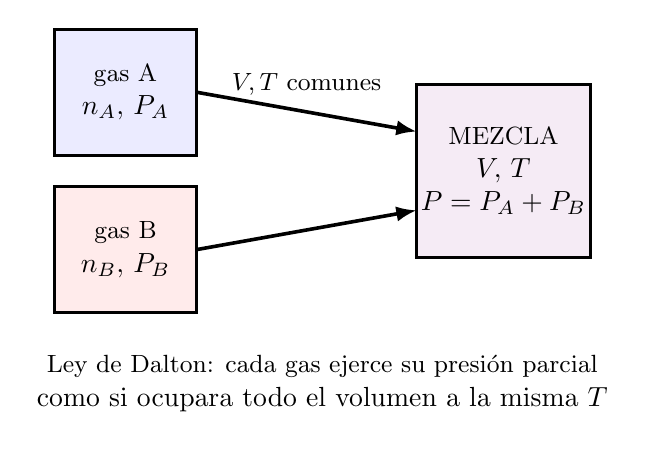
\begin{tikzpicture}[line width=1pt,>={Latex[length=2.6mm]}]
  % gas A
  \fill[blue!8] (0,2.0) rectangle (1.8,3.6); \draw[line width=1.1pt] (0,2.0) rectangle (1.8,3.6);
  \node[align=center] at (0.9,2.8){\small gas A\\$n_A,\,P_A$};
  % gas B
  \fill[red!8] (0,0) rectangle (1.8,1.6); \draw[line width=1.1pt] (0,0) rectangle (1.8,1.6);
  \node[align=center] at (0.9,0.8){\small gas B\\$n_B,\,P_B$};
  % mezcla
  \fill[blue!8] (4.6,0.7) rectangle (6.8,2.9);
  \fill[red!8] (4.6,0.7) rectangle (6.8,2.9);
  \fill[violet!8] (4.6,0.7) rectangle (6.8,2.9); \draw[line width=1.1pt] (4.6,0.7) rectangle (6.8,2.9);
  \node[align=center] at (5.7,1.8){\small MEZCLA\\$V,\,T$\\$P=P_A+P_B$};
  % flechas
  \draw[->,line width=1.3pt] (1.8,2.8)--(4.6,2.3);
  \draw[->,line width=1.3pt] (1.8,0.8)--(4.6,1.3);
  \node at (3.2,2.9){\small $V,T$ comunes};
  \node[align=center] at (3.4,-0.9){\small Ley de Dalton: cada gas ejerce su presión parcial\\ como si ocupara todo el volumen a la misma $T$};
\end{tikzpicture}
\end{document}
